\chapter{Ground State Structures for Molecular Crystals and Liquids}
\label{sec:structure}

As we lower the temperature, the properties of a condensed phase become increasingly dominated by the arrangement of molecules corresponding to the local potential energy minima, the ground state. In the same way the structure and dynamics of a small molecule can be inferred from its ground state structure, these properties can be inferred from the ground state of these condensed phases with thousands of molecules.

In this chapter we address: What are the structures and energies of the most stable crystal structures of our molecules? The problems with generic measures of order in molecular systems? What degree of ordering is present in the ground states of our molecular liquids?

\section{The Most Stable Crystal Phase}

The most stable crystal phase, for our purposes, is the crystal that will form spontaneously from the liquid phase upon cooling. Since by design this process is slow or unobservable for the molecular liquids we are using we need to use other means to identify the most stable crystal phase (described below). Of most stable crystal phases~\figref{crystals} the \dcon and \tri molecules have unit cells in the p2 wallpaper group in which the majority of crystals lie~\cite{plass:07,jennings:15}. While the \done molecule is contained in the p2mg wallpaper group which contains very few crystal structures, making it an interesting crystal structure.

\begin{figure}
    \centering
    \begin{subfigure}[t]{0.45\linewidth}
        \includegraphics[width=\textwidth]{{{Snowman-0.4-0.637556-1.00-p2mg-frame}}}
        \caption{}
        \label{fig:crystal done}
    \end{subfigure}\hfill
    \begin{subfigure}[t]{0.45\linewidth}%
        \includegraphics[width=\textwidth]{{{Snowman-0.4-0.637556-1.637556-p2-frame}}}
        \caption{}
        \label{fig:crystal dcon}
    \end{subfigure}
    \begin{subfigure}{0.45\linewidth}
        \includegraphics[width=\textwidth]{{{Trimer-0.4-0.637556-1.00-120-p2-frame}}}
        \caption{}
        \label{fig:crystal tri}
    \end{subfigure}
    \caption{The stable crystal forms of the \done~\subfigref{crystal done}, \dcon~\subfigref{crystal dcon}, and \tri~\subfigef{crystal tri} phases for each molecule. The molecules are coloured according to their orientation. The unit cell is indicated by a black box with an inversion center marked with a red dot.}
    \label{fig:crystals}
\end{figure}

The crystal structures shown in \textfigef{crystals} were determined to be the most stable crystal structures using a variety of techniques. As a starting point we wanted to find the lowest energy crystal structures, since using molecular dynamics was not possible we had to use an alternate method. By approximating our particles as hard discs and finding the closest packed structure we are able to use the isopointal search algorithm developed by~\textcite{husdon:10} to search the reduced packing space, generating a best packed structure for each wallpaper group.

The best packed structures can then be used as the starting configurations for a molecular dynamics simulation to find the lowest energy ground state~\tabref{crystal energies}. The \done and \dcon molecules have configurations with a ground state significantly lower than any other, p2mg and p2 respectively. For these two molecules we can be fairly certain these are the most stable ground state, however for the \tri molecule there are three configurations p2, p2gg and pg all with similar ground state energies.

 
\begin{table}
    \sisetup{
        table-format = +3.4,
        table-omit-exponent,
        fixed-exponent =-4,
        parse-numbers=true,
        scientific-notation=true,
        round-mode=places,
        round-precision=3}
    \centering
    \begin{tabular}{ | l | S  S  S | }
        \hline
        {Crystal} & \multicolumn{3}{c|}{Energy per molecule (\num{e-4})} \\
            &\done & \dcon & \tri \\ \hline
        p2 & 0.00001376280055& {\cellcolor{blue!20}}0.0001527208398& {\cellcolor{blue!10}}-0.0003934685913\\
        p2mg & {\cellcolor{blue!20}}0.000005732595806& 0.0004479052484& -0.0003354198174\\
        p2gg & 0.00002632511042& 0.0001699363766& {\cellcolor{blue!20}}-0.000401823091\\
        pg & 0.00002824743917& 0.0002860863393& {\cellcolor{blue!10}}-0.0004000561542\\
        p3 & 0.00003468842645& 0.0002424453316& -0.0003292839541\\
        \hline
    \end{tabular}
    \caption{The energy per molecule for a variety of the best packing crystal structures. Both the \done and \dcon systems have an arrangement with significantly lower energy, p2mg and p2 respectively. While the \tri system has three arrangements with very similar energies, the p2, p2gg and pg wallpaper groups.}
    \label{tab:crystal energies}
\end{table}

With multiple structures of the \tri molecule having similar energies further analysis is required to determine the most stable structure, for this we looked to a two phase system as described in \textsecref{two phase}. The two phase system~\figref{tri two phase} showed a rearrangement of molecules from the p2gg structure, which had the lowest ground state energy, to the p2 structure. The most likely reason for this phase transition from p2gg structure is an increased entropy in the p2 structure, hence thermodynamic stability at higher temperatures. From this analysis the p2 structure was considered the most stable structure.


\begin{figure}
    \begin{subfigure}[t]{0.5\textwidth}
        \includegraphics[width=\textwidth]{{{Trimer-1.30-0.637556-1.00-120-p2gg-1-frame-0000000000}}}
        \caption{Initial}
        \label{fig:tri rearr init}
    \end{subfigure}
    \begin{subfigure}[t]{0.5\textwidth}
        \includegraphics[width=\textwidth]{{{Trimer-1.30-0.637556-1.00-120-p2gg-1-frame-0320000000}}}
        \caption{Final}
        \label{fig:tri rearr fine}
    \end{subfigure}
    \caption{The initial~\subfigref{tri rearr init} and final~\subfigref{tri rearr fine} configurations of a two phase simulation of the \tri molecule below the melting point. We can see the solid state phase transition from a p2mg structure with four layers in each unit cell to a structure that alternates between the p2 structure (two layers) and the p2gg structure (4 layers).}
    \label{fig:tri two phase}
\end{figure}

In light of the \tri molecule having a stable structure that did not have the lowest energy ground state we performed melting point analysis on the \done and \dcon molecules. The melting points for each crystal were obtained using a two phase system~\tabref{melting}. These results confirmed the lowest energy structures were the most stable having significantly higher melting points.

\begin{table}
    \centering
    \begin{tabular}{| l l | S |}
        \hline
        Molecule & Crystal & {Melting Point} \\ \hline
        \multirow{3}{*}{\done} & p2 & 0.65 \\
                               & p2gg & 0.55 \\
                               & p2mg & 0.92 \\ \hline
        \multirow{2}{*}{\dcon} & p2 & 1.85 \\
                               & p2gg & 1.50 \\ \hline
    \end{tabular}
    \caption{Melting points of the crystal phases established from two phase systems.}
    \label{tab:melting}
\end{table}

\section{Quantifying Order in Molecular Systems}

In most cases it is fairly easy to distinguish a crystal from an amorphous phase by simple visual inspection of the two configurations. Much harder to determine visually is to quantify the degree to which a system is ordered, a problem with application in crystal growth. In this section we investigate a number of measures of order, including local order, as well as problems associated with each.

We will be investigating the order parameters using an amorphous \scon structure and a crystalline \scon structure.

2D correlation functions taking the radial distribution function at each angle

G(r)

Orientational order

\subsection{Problems with Generic Descriptions of Order in Molecular Systems}

The \dcon molecule was chosen for being a special case, this ratio of hard discs will form a compact packing~\appref{compact packing}. If we start with the compact packing of discs~\figref{compact} we can assign bonds between large and small particles to form molecules without modifying the underlying structure. Two examples of this assignment of bonds, an orientationally ordered p2 structure~\figref{ordered-frame} and an orientationally disordered random assignment of bonds~\figref{random-frame}. Both these structures have the same underlying structure of particles, despite the orientational disorder in the randomly assigned configuration it is indisputably crystalline in character and any order parameter should reflect this.

\begin{figure}
    \centering
    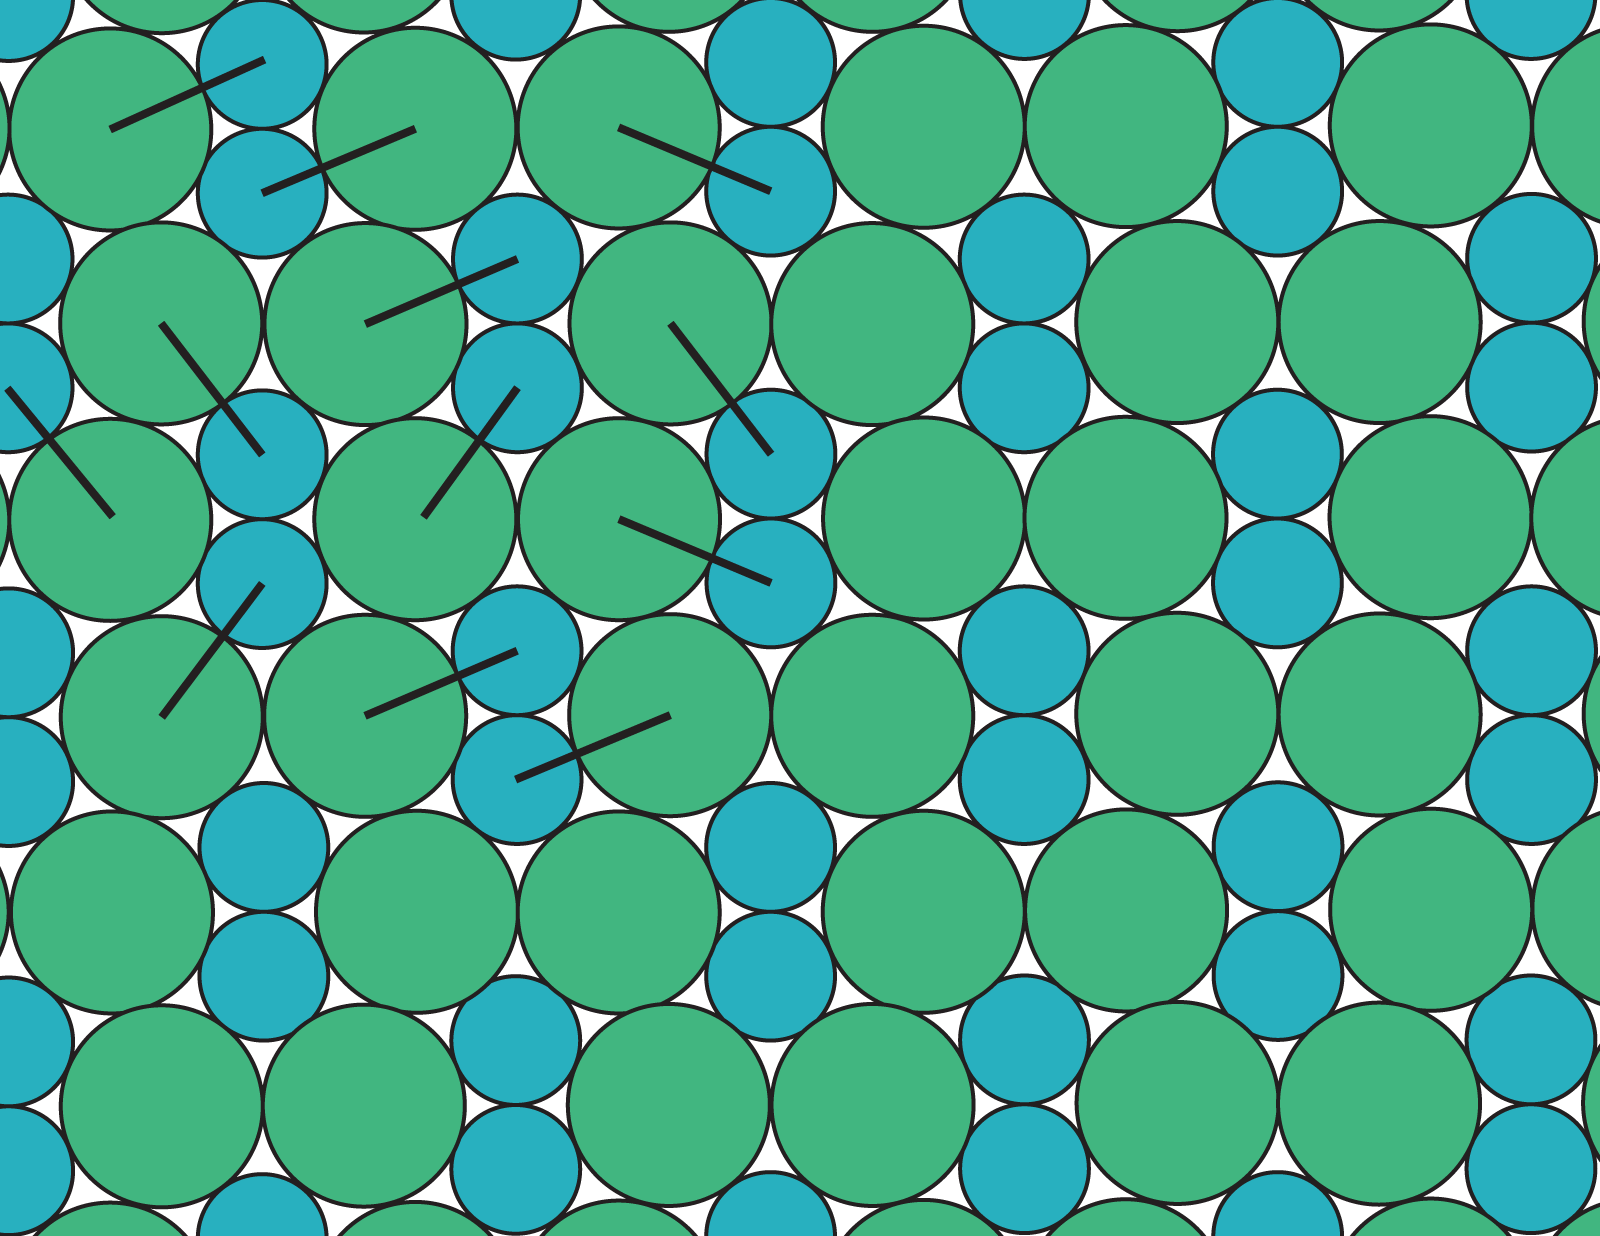
\includegraphics[width=0.5\textwidth]{compact}
    \caption{The compact packing of discs with ratio 1:0.637556. Assignment of bonds to this structure can be performed randomly (top left) with no alteration of the underlying structure.}
    \label{fig:compact}
\end{figure}

\begin{figure}
    \begin{subfigure}[t]{0.5\linewidth}
        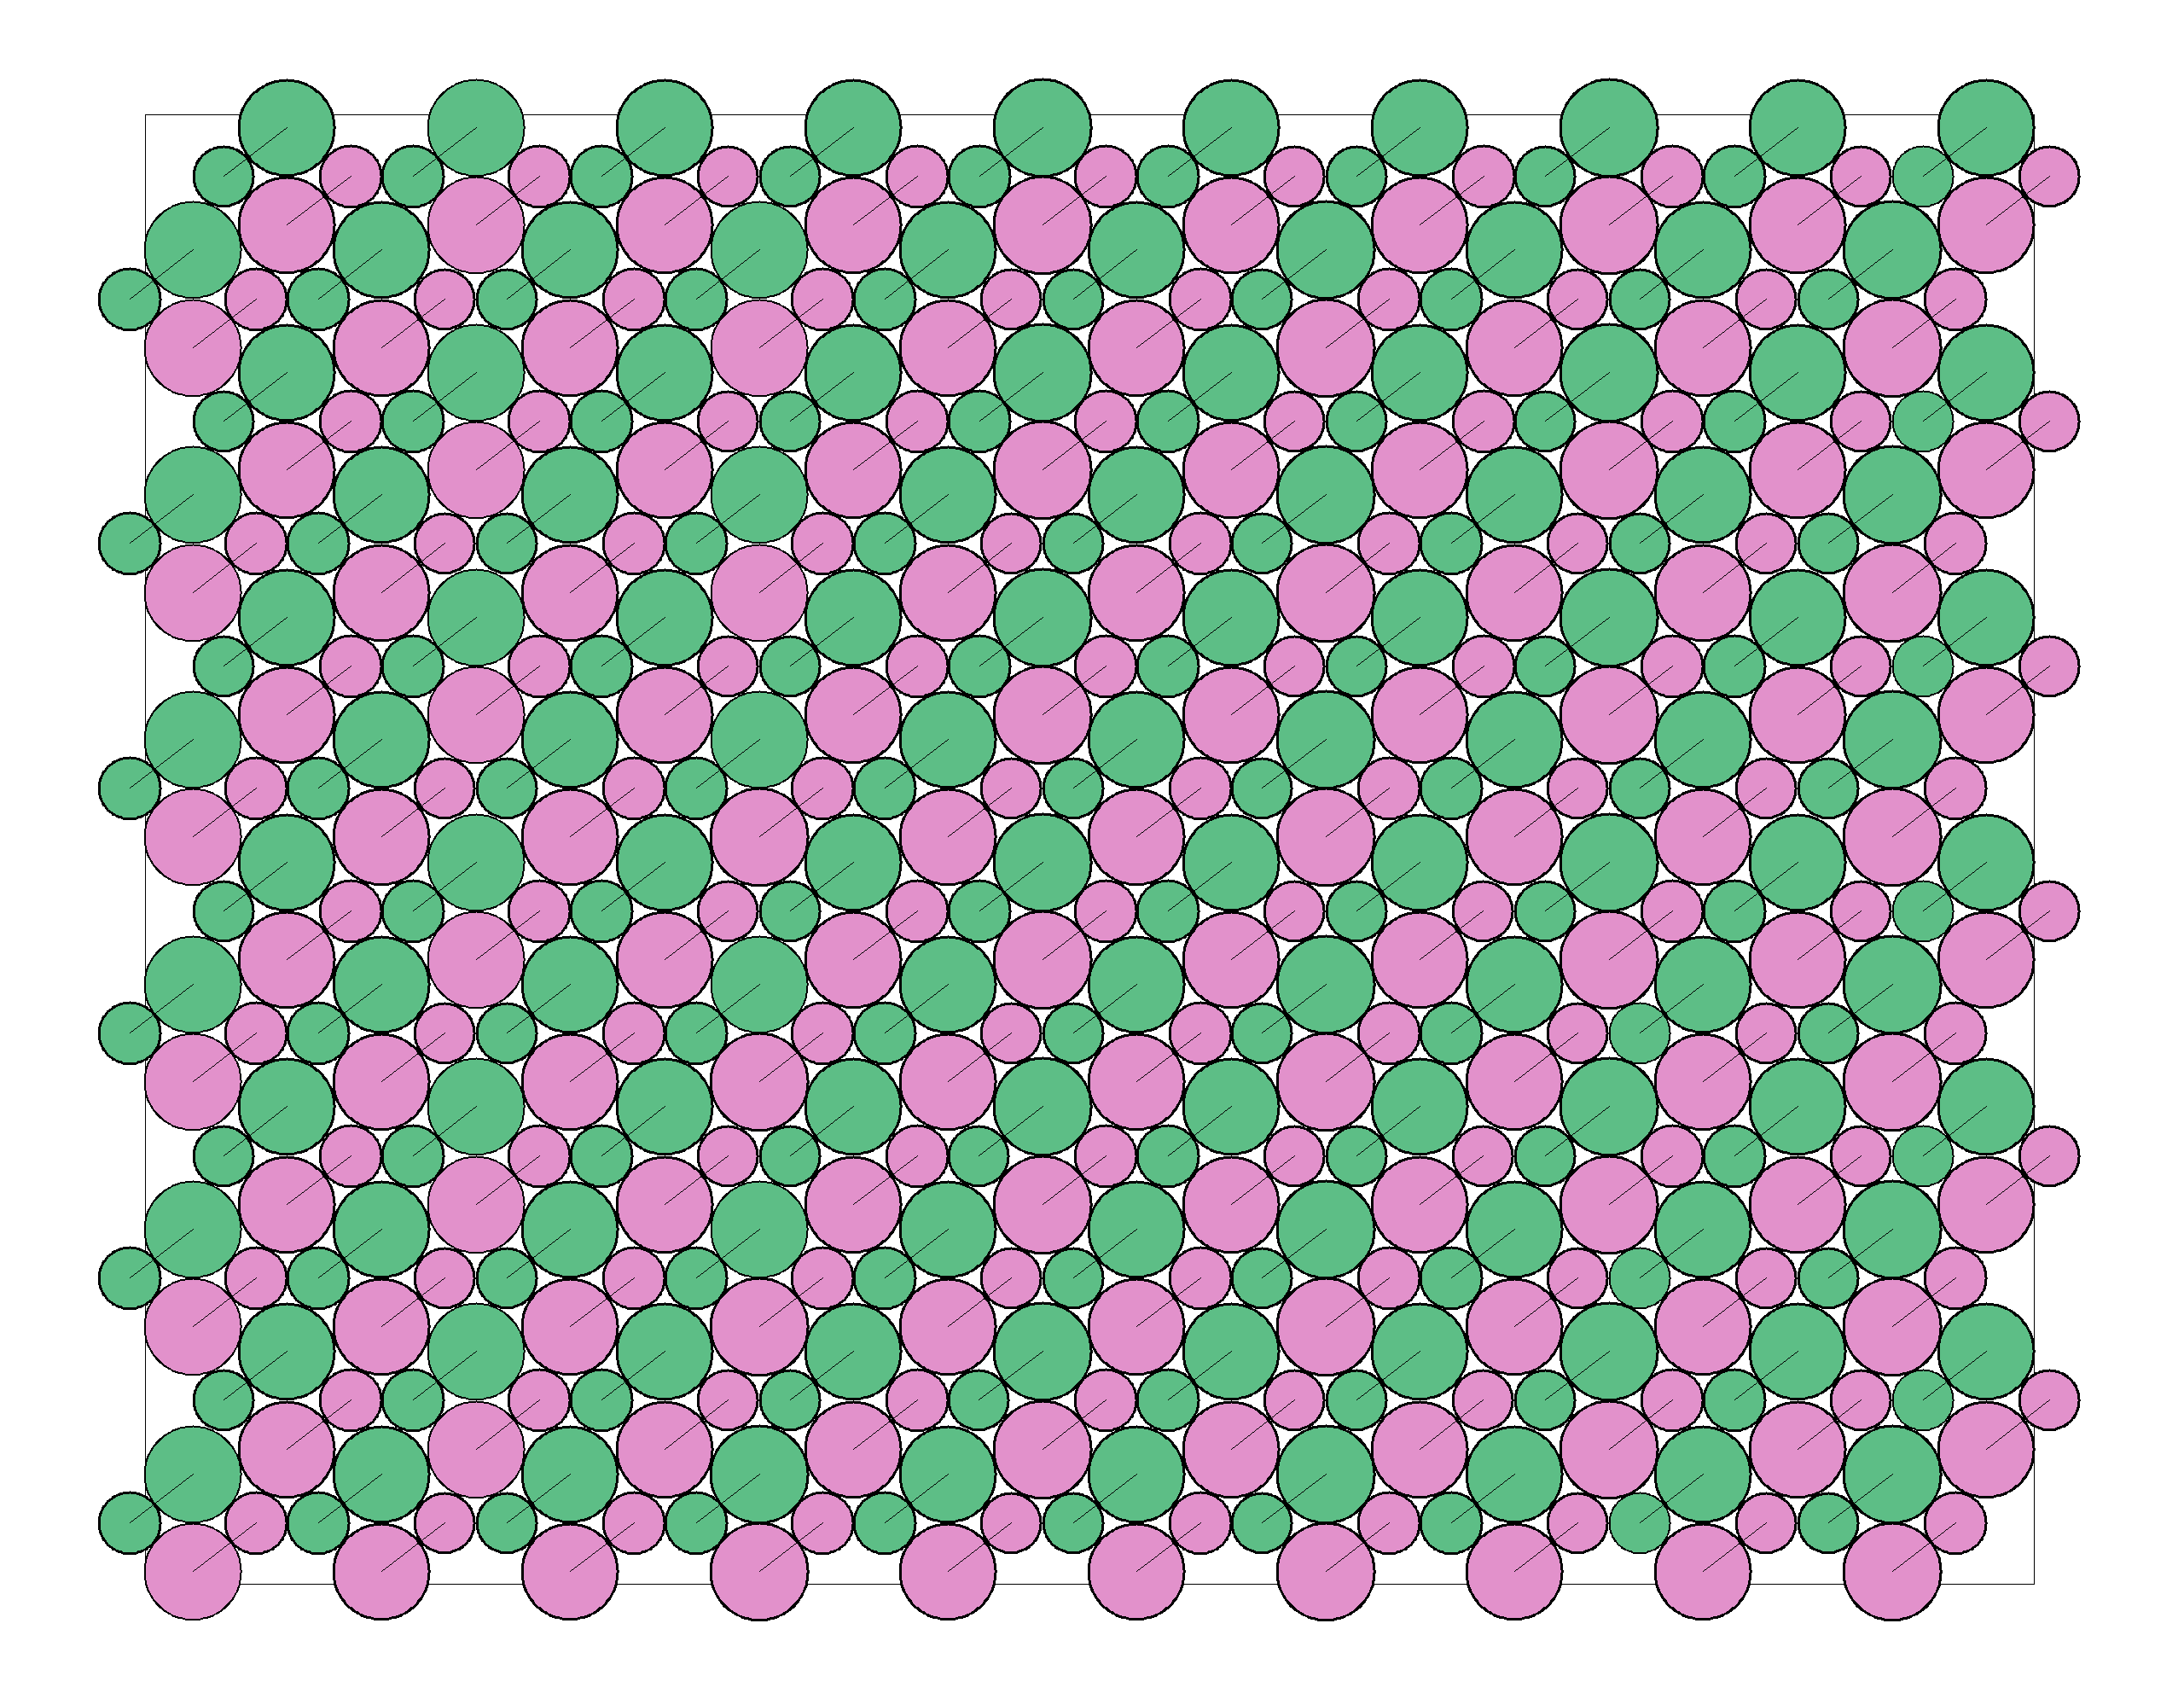
\includegraphics[width=\linewidth]{ordered-frame}
        \caption{A configuration of the \dcon molecule with p2 ordering.}
        \label{fig:ordered frame}
    \end{subfigure}
    \begin{subfigure}[t]{0.5\linewidth}
        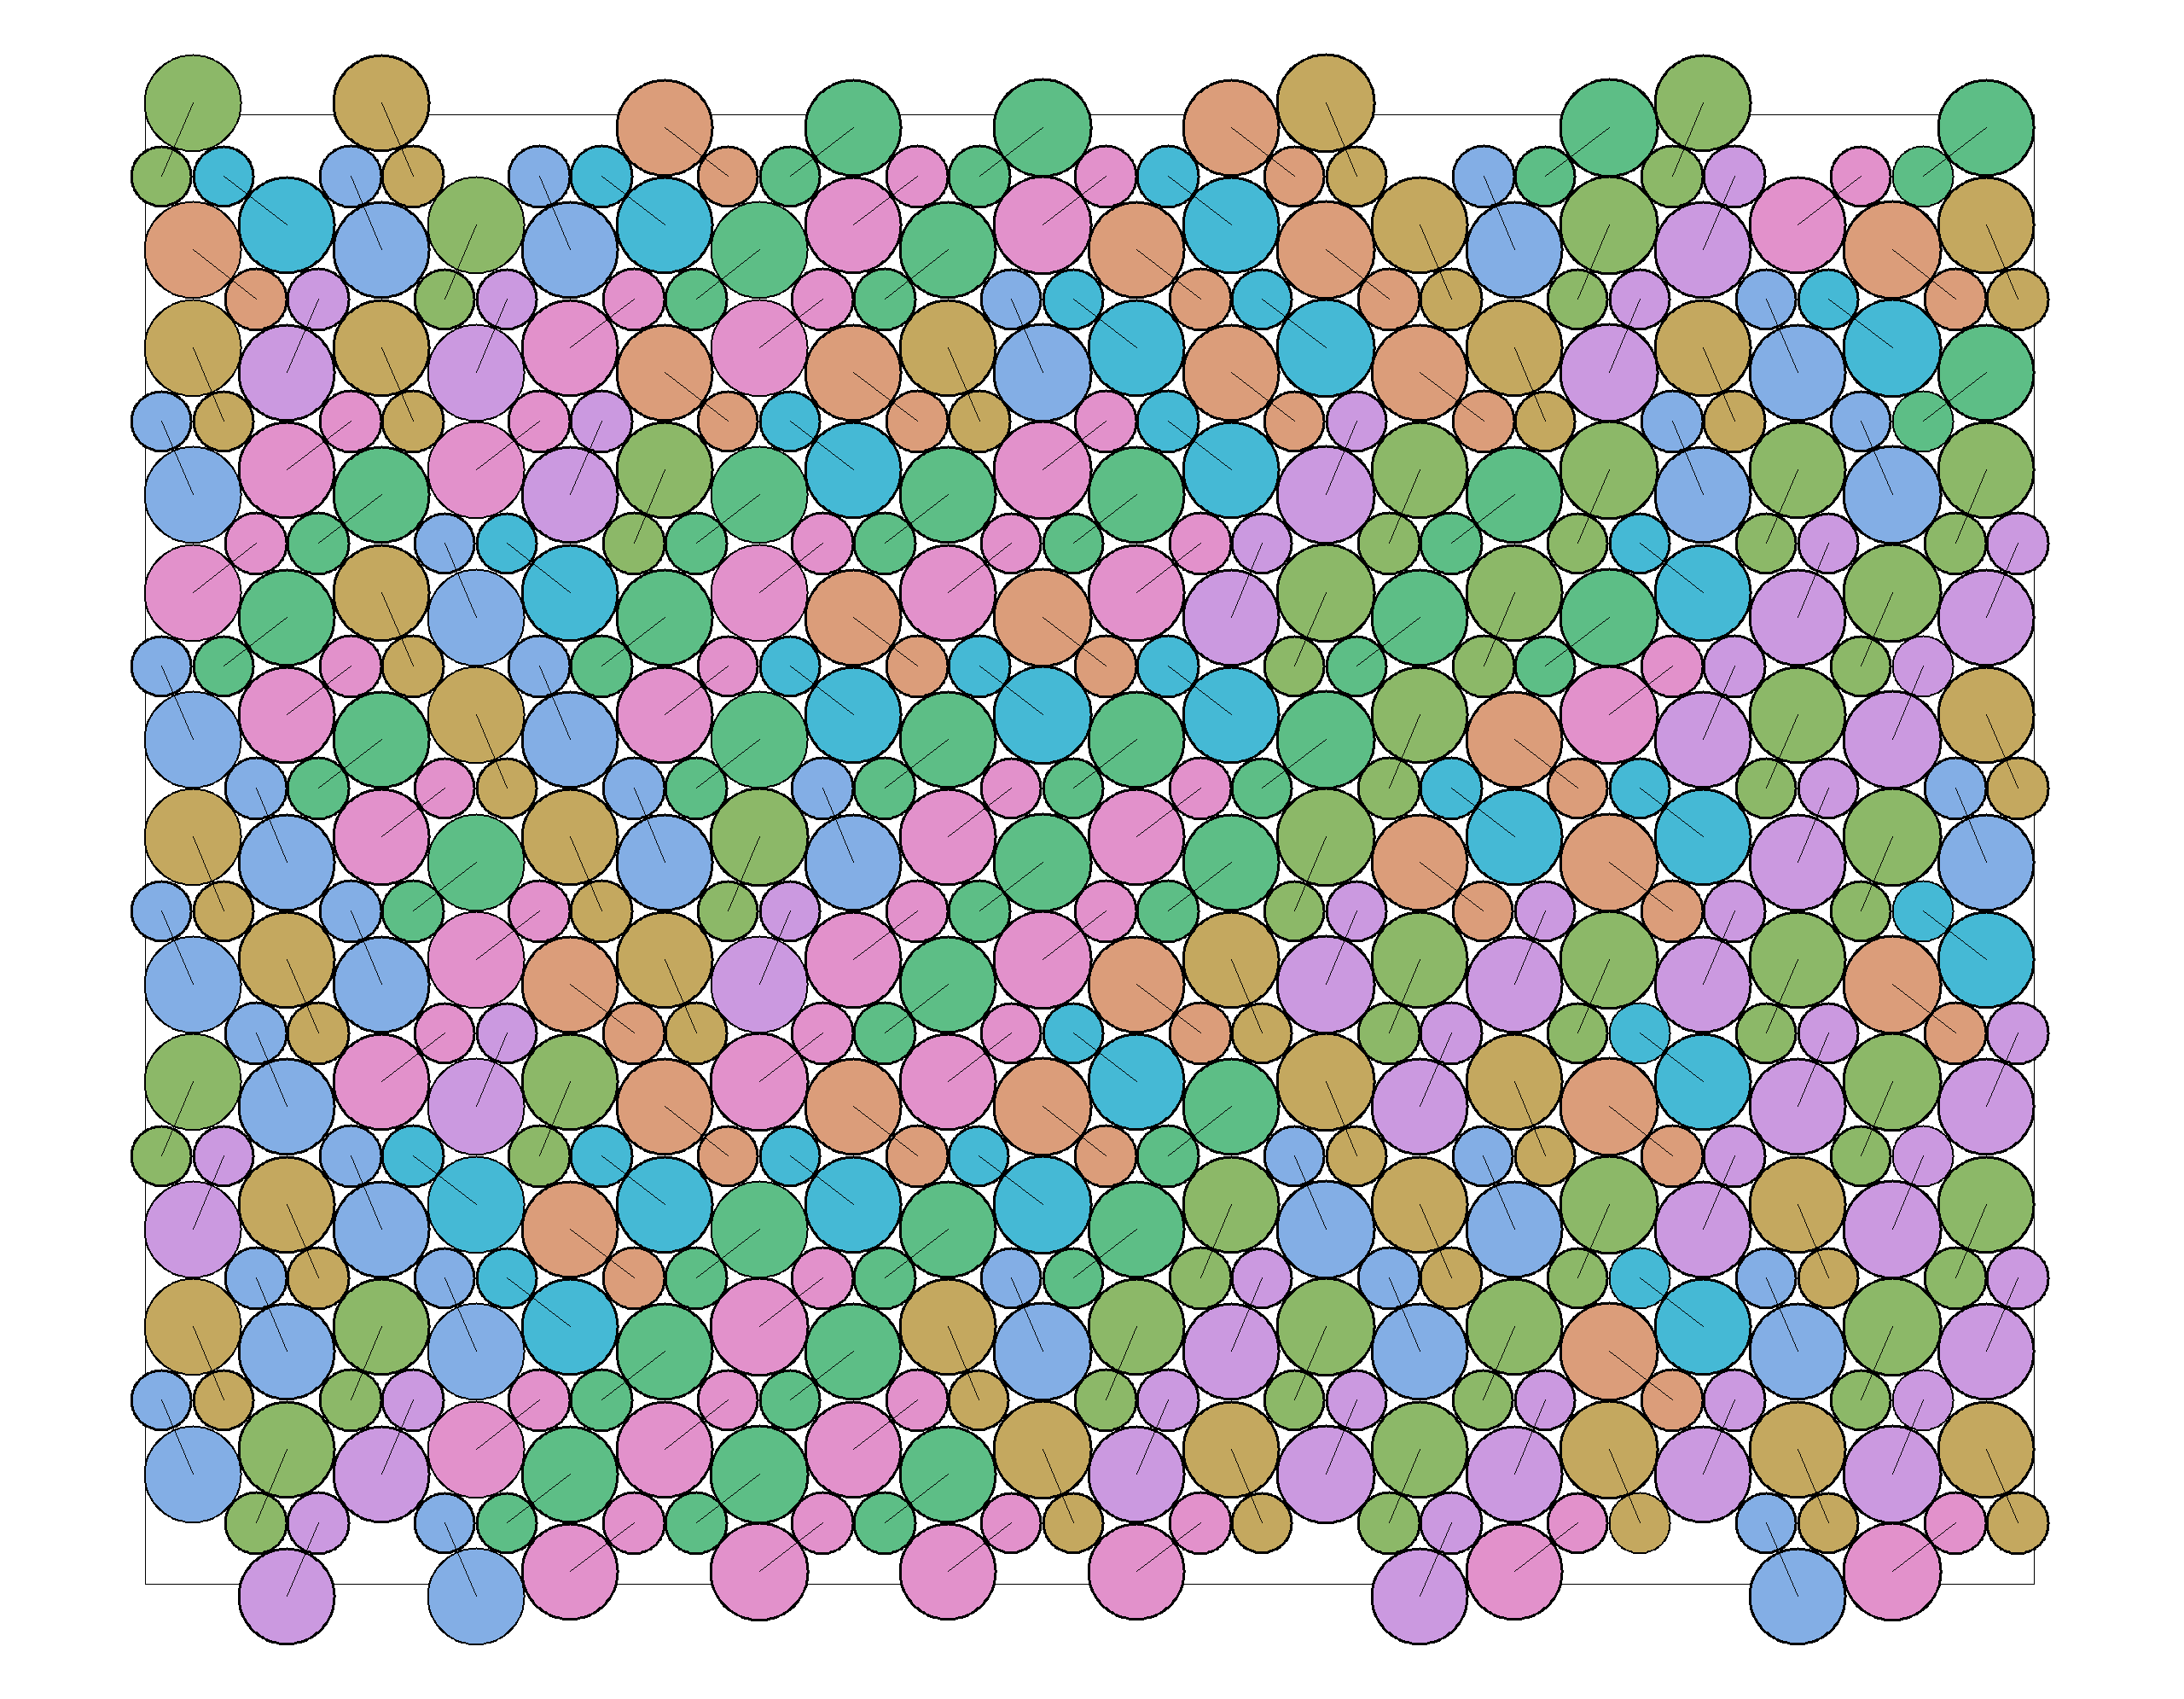
\includegraphics[width=\linewidth]{random-frame}
        \caption{A configuration of the \dcon molecule in which the bonds have been assigned randomly.}
        \label{fig:random frame}
    \end{subfigure}
    \begin{subfigure}[t]{0.5\linewidth}
        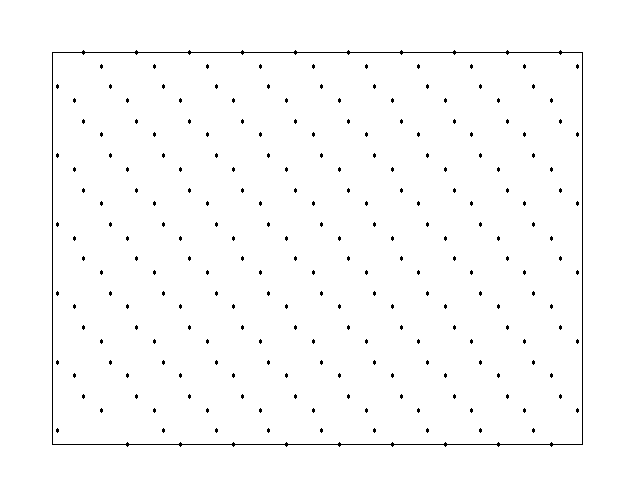
\includegraphics[width=\linewidth]{ordered-com}
        \caption{The COM of the \dcon molecule align when the configuration is crystalline.}
        \label{fig:ordered com}
    \end{subfigure}
    \begin{subfigure}[t]{0.5\linewidth}
        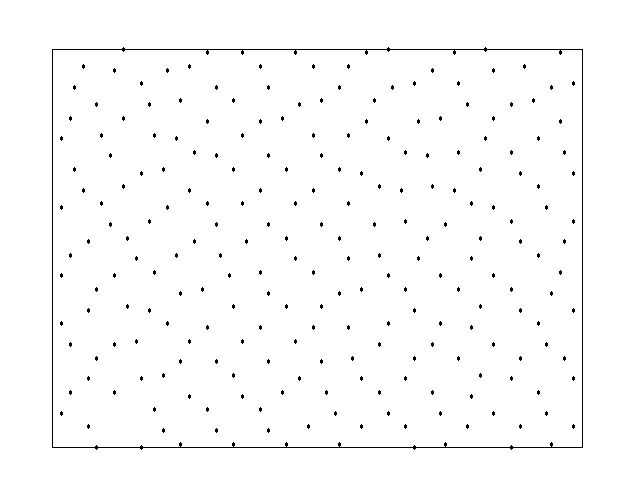
\includegraphics[width=\linewidth]{random-com}
        \caption{In the random configuration the COM of the \dcon molecule appear disordered.}
        \label{fig:random com}
    \end{subfigure}
    \begin{subfigure}[t]{0.5\linewidth}
        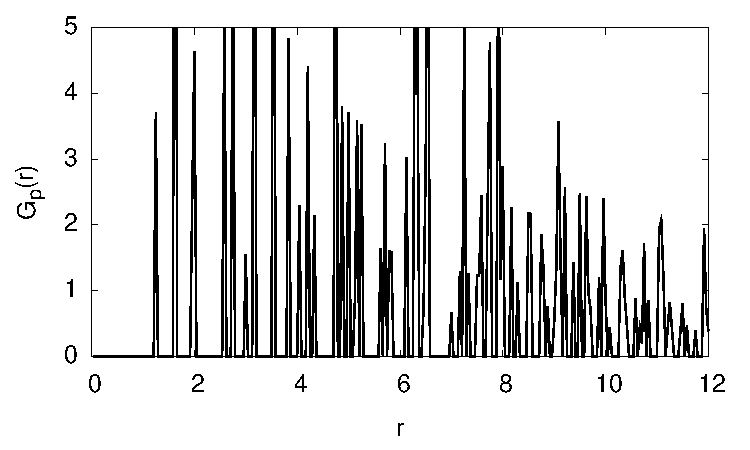
\includegraphics[width=\linewidth]{ordered-radial-part}
        \caption{The radial particle distribution function shows clear crystalline order in the sharp peaks.}
        \label{fig:ordered radial part}
    \end{subfigure}
    \begin{subfigure}[t]{0.5\linewidth}
        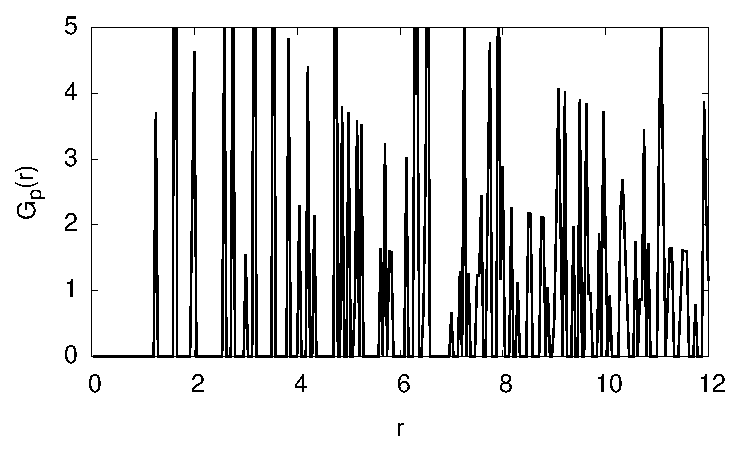
\includegraphics[width=\linewidth]{random-radial-part}
        \caption{The radial particle distribution function is essentially identical to the ordered structure.}
        \label{fig:random radial part}
    \end{subfigure}
    \caption{Comparison of the \dcon molecule with crystalline p2 ordering (left column) and random assignment of bonds (right column).}
    \label{fig:compact bonds}
\end{figure}

Solution


\subsection{Locality of Order}

We have the radial distribution functions and the orientational order parameters that inform us of order in the bulk. However these order parameters do not provide information on where the order is located, how many molecules are in these areas, whether there is a single crystal or is polycrystalline, and the size of any regions of order; a local order parameter can address all these problems. To take a local approach to order we have to find new order parameters that are capable of defining local order.

For the \done molecule we can define a local order parameter $O_\done$ based on the p2mg crystal structure as
\begin{equation}
    O_{\done} = \frac{1}{N_{\text{neigh}}}\sum_{i=1}^{N_\text{neigh}} (\vect{\hat e} \cdot \vect{\hat e_i})^2
\end{equation}
where $N_\text{neigh}$ is the number of neighbours, $\vect{\hat e}$ is the unit orientation vector of the molecule and $\vect{\hat e_i}$ is the unit orientation vector of each neighbour. Molecules that are above a cutoff of $0.8$ are considered to be crystalline while molecules below this cutoff are classed as amorphous. \textfigref{done inherent} demonstrates this order parameter using the inherent structure of the \done molecule studied throughout this chapter. There are many small regions of crystalline order while most of the configuration is amorphous.

In defining a local order parameter for the \dcon molecules we can use the particle approach that worked well for the global order parameter, however in this case we are looking at the local environment of each particle. In the p2 crystalline structure each small particle has one other small neighbour and four large neighbours, and each large particle has three small and three large neighbours. Molecules consisting of particles that have these specific neighbours are considered ordered.

The \tri molecule we are treating in the same way as the \done molecule, using the local orientational order of each molecule to assess the degree of ordering. For the \tri molecule the cutoff for this function was determined to be \num{0.7}, giving good differentiation between the crystal and liquid phases with an acceptable level of false positives and false negatives.

\section{The Structure in Amorphous Ground States}

G(r) for each
\begin{figure}
    \centering
    \begin{subfigure}[t]{0.45\linewidth}
        \includegraphics[width=\linewidth]{{{Snowman-0.80-0.637556-1.0-radial}}}
        \caption{Radial distribution of \done molecule. The broad peaks out a distance of 12 indicate long range weak medium range ordering in the inherent structure.}
        \label{fig:done radial}
    \end{subfigure}\hfill
    \begin{subfigure}[t]{0.45\linewidth}
        \includegraphics[width=\linewidth]{{{Snowman-1.55-0.637556-1.637556-radial}}}
    \caption{Radial distribution of the \dcon molecule. The initial peaks are incredibly sharp showing strong short range ordering, however this order only extends to the second shell.}
        \label{fig:dcon radial}
    \end{subfigure}
    \begin{subfigure}{0.45\linewidth}
        \includegraphics[width=\linewidth]{{{Trimer-1.05-0.637556-1.00-120-radial}}}
        \caption{Radial distribution of the \tri molecule. All the peaks for this molecule are very broad, even in the first shell.}
        \label{fig:tri radial}
    \end{subfigure}
    \caption{Radial distribution function for each molecule showing a range of types of order.}
    \label{fig:radial distributions}
\end{figure}

G_part(R) for each

\begin{figure}
    \centering
    \begin{subfigure}[t]{0.45\linewidth}
        \includegraphics[width=\linewidth]{{{Snowman-0.80-0.637556-1.0-radial_part}}}
        \caption{Radial particle distribution function for the \done molecule.}
        \label{fig:done radial part}
    \end{subfigure}\hfill
    \begin{subfigure}[t]{0.45\linewidth}
        \includegraphics[width=\linewidth]{{{Snowman-1.55-0.637556-1.637556-radial_part}}}
        \caption{Radial particle distribution function for the \dcon molecule. This figure shows the presence of medium range ordering in the peaks extending out to a distance of 12.}
        \label{fig:dcon radial part}
    \end{subfigure}
    \begin{subfigure}{0.45\linewidth}
        \includegraphics[width=\linewidth]{{{Trimer-1.05-0.637556-1.00-120-radial_part}}}
        \caption{Radial particle distribution function for the \tri molecule.}
        \label{fig:tri radial part}
    \end{subfigure}
    \caption{Radial particle distribution for the three molecules.}
    \label{fig:radial part distributions}
\end{figure}
Local order of each

\begin{figure}
    \centering
    \begin{subfigure}[t]{0.45\linewidth}
        \includegraphics[width=\textwidth]{{{Snowman-0.80-0.637556-1.0-frame-0320000191}}}
        \caption{The configuration of \done shows regions of orientational order with layers of molecules arranged antiparallel to each other. These regions have different orientations indicating a series of nucleation events.}
        \label{fig:done inherent}
    \end{subfigure}\hfill
    \begin{subfigure}[t]{0.45\linewidth}
        \includegraphics[width=\textwidth]{{{Snowman-1.55-0.637556-1.637556-frame-0320000182}}}
        \caption{The \dcon molecule shows no sign of long range order. There are small clusters of particles exhibiting the orientationally disordered crystalline phase, however these only exhibit local interactions.}
        \label{fig:dcon inherent}
    \end{subfigure}
    \begin{subfigure}{0.45\linewidth}
        \includegraphics[width=\textwidth]{{{Trimer-1.00-0.637556-1.00-120-frame-0320000177}}}
        \caption{The \tri molecule shows no sign of ordering, a truly amorphous phase.}
        \label{fig:tri inherent}
    \end{subfigure}
    \caption{Final inherent structure configurations for each molecule, the colouring of the molecules representative of their orientations.}
    \label{fig:inherent structures frame}
\end{figure}
% End of structure

The radial distribution function $G(r)$ is one of the general techniques for detecting ordering in a simulated system. It is a distribution of the distances between the molecular centers of mass. The radial distribution of the \done molecule~\figref{done radial} shows an intense first shell peak, the immediate neighbours are at well defined distances. This order extends out to 12 units distance with \done molecule exhibiting broad peaks, indicating the presence of some weak medium-range ordering. The \dcon molecule~\figref{dcon radial} exhibits an intense first peak and some sharp secondary and second shell peaks. The intensity and sharpness of these peaks can be attributed to the interactions of the \dcon molecules as the concavity. The \dcon molecule has the largest concavity of the three molecules and when molecules are in the concavity they are highly constrained giving tight distributions of the center of mass~\figref{dcon radial part}. Unlike the sharp peaks of the \dcon molecule the \tri molecule~\figref{tri radial} has a series of three broad peaks in the first shell of neighbours, with order only extending to three broad peaks in the second shell. It is likely the concavities of the \tri molecule are much less selective than the concavities of the dimers.


\begin{figure}
    \centering
    \includegraphics[width=0.45\textwidth]{{{Snowman-1.55-0.637556-1.637556-radial2d_rel}}}
    \caption{The two dimensional radial distribution of the \dcon molecule in which the intensity of the peak is indicated by the amount of blue. The intense inner peaks (circled in red) show the distribution of the COM when the molecules interact via the concavity.}
    \label{fig:dcon radial2d_abs}
\end{figure}

Another measure of order is to look at the orientational distribution of the molecules. This provides an alternate look at the degree to which molecules are organising over large distances. The angular distribution looks at whether there are some directions which molecules are favouring, an indicator of long range ordering. None of the molecules~\figref{angular distributions} show a directional preference, a sign that there is no long range orientational ordering taking place.

\subsection{Order in \dcon}

Both of the previous methods of describing order use properties of the molecule, the orientation and center of mass. In molecular systems these properties can fail to reflect the underlying structure. Consider the compact binary packing with a size ratio of 1:0.637556~\figref{compact}, an arrangement equivalent to packing the \dcon molecule without the allocation of bonds. The allocation of bonds can be performed randomly with no adjustment to the structure of the underlying particles. Two examples of assigning bonds; an ordered p2 structure~\figref{ordered frame}, and a randomly oriented structure~\figref{random frame} demonstrate the issues in identifying order with a random assignment of bonds. The orientational order of the p2 structure can easily be seen with diagonal banding of colours, corresponding to the two orientations present in the structure while the randomly assigned structure has molecules arranged with no orientational order, distributed between the eight possible molecular orientations. We can attempt to remove the noise of this orientational disorder by only plotting the centers of mass~(\textfigref{ordered com} and~\textfigref{random com}), however this gives a very similar result, the ordered structure exhibits distinctly crystalline behaviour with centers of mass aligning in rows while the random structure needs further analysis to be considered ordered.


In the randomly oriented configuration the molecules are a construct placed on an ordered arrangement of particles. Since it is the particles define the order rather than the molecules, using an order parameter that is a measure of the ordering of the particles rather than the molecules is more appropriate for this molecule. If we define the \emph{particle radial distribution function} $G_p(r)$ in the same way as the radial distribution function, however instead of centers of mass we use the centers of density, the center of each disc. This particle radial distribution function translates better to experiments which look at the centers of density, each atom, rather than centers of mass. 



Using this particle radial distribution function we can look for order in the inherent structures of the molecules. The \dcon molecule~\figref{dcon radial part} shows medium range ordering which was not present on the radial distribution function~\figref{dcon radial}. The particle radial distribution function has also helped in reducing the number of secondary peaks with much sharper and higher intensity peaks. The \done molecule~\figref{done radial part} shows no medium range ordering unlike when using the radial distribution~\figref{done radial} which is an demonstrates the specificity of detecting order in these molecules. To get the best results order parameters need to be tailored to the particular molecule.


\section{Locality of Order}

